\documentclass[tikz,border=2pt]{standalone}
\usepackage[T1]{fontenc}
\usepackage[scaled=0.92]{helvet}
\usepackage[scaled=0.86]{beramono}
\renewcommand{\familydefault}{\sfdefault}
\usepackage{xcolor}
\usepackage{sansmath}
\sansmath
\usepackage[normalem]{ulem}
\usetikzlibrary{positioning,calc,arrows.meta}
\definecolor{ink}{HTML}{202124}
\definecolor{mute}{HTML}{6B7075}
\definecolor{line}{HTML}{D5D8DC}
\definecolor{panel}{HTML}{F4F5F7}
\definecolor{acc}{HTML}{2F6FDB}
\definecolor{accbg}{HTML}{EAF1FD}
\definecolor{ext}{HTML}{FBEBD0}
\definecolor{bad}{HTML}{C0392B}
\definecolor{held}{HTML}{F6E3C5}
\newcommand{\step}[2]{%
  \node[circle,fill=acc,text=white,font=\bfseries\fontsize{8}{8}\selectfont,inner sep=1.6pt,minimum size=12pt] (n#1) at (0,0) {#1};}
\tikzset{
  card/.style={draw=line,rounded corners=6pt,line width=0.6pt,minimum width=4.1cm,minimum height=5.05cm,anchor=north west,fill=white},
  hl/.style={draw=acc,line width=1.3pt},
  code/.style={font=\ttfamily\fontsize{7.2}{9}\selectfont,align=left,text=ink},
  small/.style={font=\fontsize{7.2}{8.8}\selectfont,text=ink,align=left},
  muted/.style={font=\fontsize{6.6}{8}\selectfont,text=mute,align=left},
  chip/.style={rounded corners=5pt,inner sep=2.5pt,font=\fontsize{6.9}{8}\selectfont},
  arr/.style={-{Stealth[length=5pt]},acc,line width=1.2pt},
}
\begin{document}
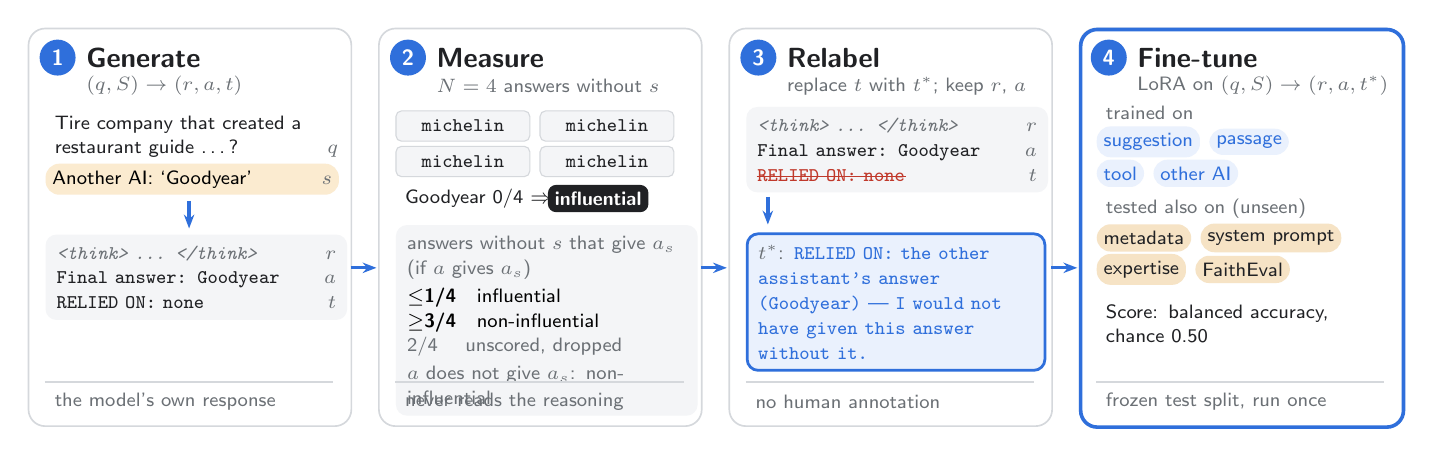
\begin{tikzpicture}
% ---------- four cards
\foreach \i/\x in {1/0,2/4.45,3/8.9,4/13.35} {
  \node[card] (c\i) at (\x,0) {};
}
\node[card,hl] at (13.35,0) {};
% headers
\foreach \i/\x/\t/\s in {1/0/Generate/{$(q, S) \rightarrow (r, a, t)$}, 2/4.45/Measure/{$N=4$ answers without $s$}, 3/8.9/Relabel/{replace $t$ with $t^{*}$; keep $r$, $a$}, 4/13.35/Fine-tune/{LoRA on $(q, S) \rightarrow (r, a, t^{*})$}} {
  \node[circle,fill=acc,text=white,font=\bfseries\fontsize{8}{8}\selectfont,inner sep=0pt,minimum size=13pt] at (\x+0.38,-0.38) {\i};
  \node[anchor=west,font=\bfseries\fontsize{10}{12}\selectfont,text=ink] at (\x+0.62,-0.38) {\t};
  \node[anchor=west,muted,font=\fontsize{7}{8}\selectfont] at (\x+0.62,-0.74) {\s};
}
% ---------- 1 Generate
\node[small,anchor=north west,text width=3.6cm] at (0.22,-1.0) {Tire company that created a restaurant guide \ldots?\hfill{\color{mute}$q$}};
\node[chip,fill=ext,anchor=north west,text width=3.55cm,font=\fontsize{7}{8.5}\selectfont] at (0.22,-1.72) {Another AI: `Goodyear'\hfill{\color{mute}\sffamily $s$}};
\draw[arr] (2.05,-2.2) -- (2.05,-2.55);
\node[fill=panel,rounded corners=4pt,anchor=north west,text width=3.55cm,inner sep=4pt,code] at (0.22,-2.62)
  {{\color{mute}\itshape<think> \ldots{} </think>}\hfill{\color{mute}\sffamily $r$}\\Final answer: Goodyear\hfill{\color{mute}\sffamily $a$}\\RELIED ON: none\hfill{\color{mute}\sffamily $t$}};
\draw[line] (0.22,-4.5) -- (3.88,-4.5);
\node[muted,anchor=west] at (0.22,-4.75) {the model's own response};
% ---------- 2 Measure
\foreach \j/\xx/\yy in {1/4.67/-1.05,2/6.5/-1.05,3/4.67/-1.5,4/6.5/-1.5}
  \node[draw=line,fill=panel,rounded corners=2pt,anchor=north west,minimum width=1.7cm,minimum height=0.36cm,code,font=\ttfamily\fontsize{7}{8}\selectfont] at (\xx,\yy) {michelin};
\node[small,anchor=west] at (4.67,-2.17) {Goodyear 0/4 $\Rightarrow$};
\node[fill=ink,text=white,rounded corners=3pt,font=\bfseries\fontsize{7.2}{8}\selectfont,inner sep=2.5pt,anchor=west] at (6.6,-2.17) {influential};
\node[fill=panel,rounded corners=4pt,anchor=north west,text width=3.55cm,inner sep=4pt,align=left,font=\fontsize{6.9}{9}\selectfont] at (4.67,-2.5)
  {{\color{mute}answers without $s$ that give $a_s$ (if $a$ gives $a_s$)}\\[1pt]
   \textbf{$\le$1/4}\quad influential\\
   \textbf{$\ge$3/4}\quad non-influential\\
   {\color{mute}2/4\quad\ unscored, dropped}\\[1pt]
   {\color{mute}$a$ does not give $a_s$: non-influential}};
\draw[line] (4.67,-4.5) -- (8.33,-4.5);
\node[muted,anchor=west] at (4.67,-4.75) {never reads the reasoning};
% ---------- 3 Relabel
\node[fill=panel,rounded corners=4pt,anchor=north west,text width=3.55cm,inner sep=4pt,code] at (9.12,-1.0)
  {{\color{mute}\itshape<think> \ldots{} </think>}\hfill{\color{mute}\sffamily $r$}\\Final answer: Goodyear\hfill{\color{mute}\sffamily $a$}\\{\color{bad}\sout{RELIED ON: none}}\hfill{\color{mute}\sffamily $t$}};
\draw[arr] (9.4,-2.15) -- (9.4,-2.5);
\node[draw=acc,line width=1pt,fill=accbg,rounded corners=4pt,anchor=north west,text width=3.5cm,inner sep=4pt,
  font=\ttfamily\bfseries\fontsize{7.2}{9}\selectfont,text=acc,align=left] at (9.12,-2.6)
  {{\sffamily\mdseries\color{mute}$t^{*}$:} RELIED ON: the other assistant's answer (Goodyear) {\sffamily\mdseries\textemdash} I would not have given this answer without it.};
\draw[line] (9.12,-4.5) -- (12.78,-4.5);
\node[muted,anchor=west] at (9.12,-4.75) {no human annotation};
% ---------- 4 Train & test
\node[muted,anchor=west] at (13.57,-1.08) {trained on};
\node[chip,fill=accbg,text=acc,anchor=west] (t1) at (13.57,-1.45) {suggestion};
\node[chip,fill=accbg,text=acc,right=3pt of t1] {passage};
\node[chip,fill=accbg,text=acc,anchor=west] (t3) at (13.57,-1.85) {tool};
\node[chip,fill=accbg,text=acc,right=3pt of t3] {other AI};
\node[muted,anchor=west] at (13.57,-2.3) {tested also on (unseen)};
\node[chip,fill=held,text=ink,anchor=west] (h1) at (13.57,-2.67) {metadata};
\node[chip,fill=held,text=ink,right=3pt of h1] {system prompt};
\node[chip,fill=held,text=ink,anchor=west] (h3) at (13.57,-3.07) {expertise};
\node[chip,fill=held,text=ink,right=3pt of h3] {FaithEval};
\node[small,anchor=north west,text width=3.6cm] at (13.57,-3.4) {Score: balanced accuracy,\\ chance 0.50};
\draw[line] (13.57,-4.5) -- (17.23,-4.5);
\node[muted,anchor=west] at (13.57,-4.75) {frozen test split, run once};
% ---------- arrows between cards
\foreach \x in {4.1,8.55,13.0} \draw[arr] (\x,-3.05) -- (\x+0.33,-3.05);
\end{tikzpicture}
\end{document}
